\documentclass[aps,prl,twocolumn,superscriptaddress,nofootinbib]{revtex4-1}

% the percent sign gives comments in Latex
% top line indicates this is for Physical Review, standard journal format,
% suitable for electronic submission of articles

% the line above is necessary to start any latex document.
% this is one variation that should work for most things.
% if you want double spaceing, use the following:
%
%\documentclass[prd,preprint,letterpaper]{revtex4}
%
% the "preprint" designation will make a wider line
% spacing, good for markup.
\usepackage{graphicx}  % this is the up-to-date package for all figures
\usepackage{amssymb}   % for math
\usepackage{verbatim}  % for the comment environment
\usepackage{color}
\usepackage{gensymb}
\usepackage{amsmath}
\usepackage{amsfonts}
\usepackage{soul}


\usepackage[section]{placeins}

\usepackage{wrapfig}
\usepackage{hyperref}
\usepackage{titlesec}
\usepackage{amssymb}   % for math
\usepackage{verbatim}  % for the comment environment
\usepackage{color}
\usepackage[nodisplayskipstretch]{setspace}
\usepackage{amsmath}
\usepackage{blindtext}
%\usepackage[pdftex]{graphicx}
\usepackage[outdir=./]{epstopdf}
\usepackage[space]{grffile}
\usepackage{epsfig}
\usepackage[separate-uncertainty=true]{siunitx}
\usepackage{tikz}
\usepackage{pgfgantt}
\usepackage[english]{babel}
\usepackage[utf8]{inputenc}

\titlespacing*{\section}
{0pt}{1\baselineskip}{.5\baselineskip}

\titlespacing*{\subsection}
{0pt}{1\baselineskip}{.3\baselineskip}

\setlength{\textfloatsep}{1\baselineskip plus 0.2\baselineskip minus 0.5\baselineskip}

\usepackage{footnote}

\bibliographystyle{apsrev}


% these are some custom control of the page size and margins
% \topmargin= 0.2in  % these 1st two may be needed for some computers
% \textheight=8.75in
%\textwidth=6.5in
%\oddsidemargin=0cm
%\evensidemargin=0cm

% this is where the actual document itself (rather than control statements) begins:

\begin{document}

% use a style that gives automatic headings
%\pagestyle{headings}



% the \title{} command generates a title.

% the \\ below is used to FORCE a line break in the middle of the sentence--
% otherwise latex computes it for you

\title{Relativistic Kinematics}


\author{\textbf{Bryan Yamashiro}}
\author{Brandon Agtarap}
\author{Corey Mutnik}
\author{Daichi Hiramatsu}
%\author{Christina Nelson}

\affiliation{Department of Physics \& Astronomy, \\
University of Hawaii at Manoa,\\
2505 Correa Rd, Honolulu, HI, 96822, USA}





	      % \section is used to start a new one with a heading
\begin{abstract}

This study aimed to understand relativistic kinematics while utilizing detector simulations in both the lab frame, and the center of mass. Two programs used in this study include the Relativistic Kinematics Program\,(RELKIN), and the Detector Simulation Program\,(DETSIM).
%The sigma deviations of LiF ranged between 0.77$\sigma$ to 1.94$\sigma$. The low sigma results showed that the lithium fluoride quite accurately determined the lattice constant. Conversely, the sodium chloride sigma errors ranged between 2.27$\sigma$ to 3.28$\sigma$, which showed more deviation, but was still acceptable.



\end{abstract}

\maketitle    % this line is necessary to tell latex you are done with all
	      % of the stuff associated with the title, and now it can go
              % ahead and generate the title portion
\section{Chapter 3}
\subsection{Question 3.4}
\begin{equation}
\sqrt{s_{p\rightarrow e}}=\sqrt{(m_p+m_e)^2+2m_e(E_p-m_p)}
\label{sproton}
\end{equation}
\begin{equation}
\sqrt{s_{e\rightarrow p}}=\sqrt{(m_p+m_e)^2+2m_p(E_e-m_e)}
\label{selectron}
\end{equation}

The subscripts in equations\,\ref{sproton}\&\ref{selectron}, \textit{p}\&\textit{e}, correlate to proton and electron,
 respectively. The subscripts on the CM\,(Center of Mass) energies\,($\sqrt{s}$) correspond to the two situations situations 
 either involving a proton colliding into the initial electron\,(p$\rightarrow$ e) and an electron colliding with a 
 stationary proton\,(e$\rightarrow$ p). The CM energy of the electron colliding into a target proton was higher in energy by 
 an order of magnitude. $\sqrt{s_{p\rightarrow e}}$ was \fbox{$9.44\times 10^{-1}$\,GeV}, and $\sqrt{s_{e\rightarrow p}}$ 
 was \boxed{4.43\,\textnormal{GeV}}.
\\
\indent The advantage of using a collider\,(beam-beam) rather than a stationary target\,(beam-target) is the total 4-momentum for both frames. Converse to the beam-target, which has a total 3-momentum equaling zero, the beam-beam contains doubled 4-momentum. The (beam-target) and (beam-beam) collisions yielded energies of \boxed{0.303\,\textnormal{GeV}} and \boxed{90.0\,\textnormal{GeV}}, respectively. This trait allows for higher energy collisions compared to a stationary hit.


\subsection{Question 3.5}
The threshold energy for producing K$^0$ mesons plus $\Lambda^0$ in pion-proton collisions is \boxed{885.7\,\textnormal{MeV}}. No other reactions could produce K$^0$ mesons plus $\Lambda^0$ other than the pion-proton collision through the RELKIN program. To produce pions, a q-value of \boxed{140.0\,\textnormal{MeV}} and momentum of \boxed{794.5\,\textnormal{MeV}} was required.
\\
\begin{equation}
\frac{s_{p\rightarrow Be}-(m_p+m_{Be})^2}{2m_{Be}}+m_p=E_p
\label{Be}
\end{equation}

 \textit{The mass of Beryllium\,(Be) used in equation\,\ref{Be}, was $1.497\times10^{-26}\,\textnormal{kg}$ or 8.364\,GeV. The threshold energy mentioned before was used for s$_{p \rightarrow Be}$, and the constants for a proton and Be. The beam energy required for a (p $\rightarrow$ Be) collision is $-$4.181\,GeV.}\footnote{This section is for reference, the corrected $(p\rightarrow p)$ is extrapolated upon}

\begin{equation}
\frac{s_{p\rightarrow p}-(m_p+m_{p})^2}{2m_{p}}+m_p=E_p
\label{Pe}
\end{equation}

\indent Equation\,\ref{Pe} represents the (p$\rightarrow$ p) collision.\footnote{Directions were not read as they state,  ``you may assume that the target is a proton".} Following the prior procedures, the beam energy required was found to be $-$0.04663\,GeV.
\\
\indent The electron and positron energy required was \boxed{1776.9\,\textnormal{MeV}/c^2}.


\subsection{Question 3.8}

\begin{equation}
\tan(\theta)=\frac{\sin(\theta^*)}{\gamma(\cos(\theta^*)+\beta/\beta^*)}
\label{tan}
\end{equation}
\begin{equation}
\theta_{max}=\frac{E^*_\nu}{E_\nu}
\label{neut}
\end{equation}

The maximum muon Lab angle was found to be \boxed{135\degree} for a momentum of 1000\,MeV with 1000 iterations. It is imperative to note that the maximum muon Lab angle changes with respect to different momentum parameters. A test was conducted with a momentum of 500\,MeV with 1000 iterations, and the muon Lab angle was \boxed{150\degree}.  The neutrino also has a maximum Lab angle represented in equation\,\ref{neut}. The equation was derived from equation\,\ref{tan}, using the relationships for $\beta$.

\subsection{Question 3.12}

\begin{figure}[h!]
\begin{center}
\centerline{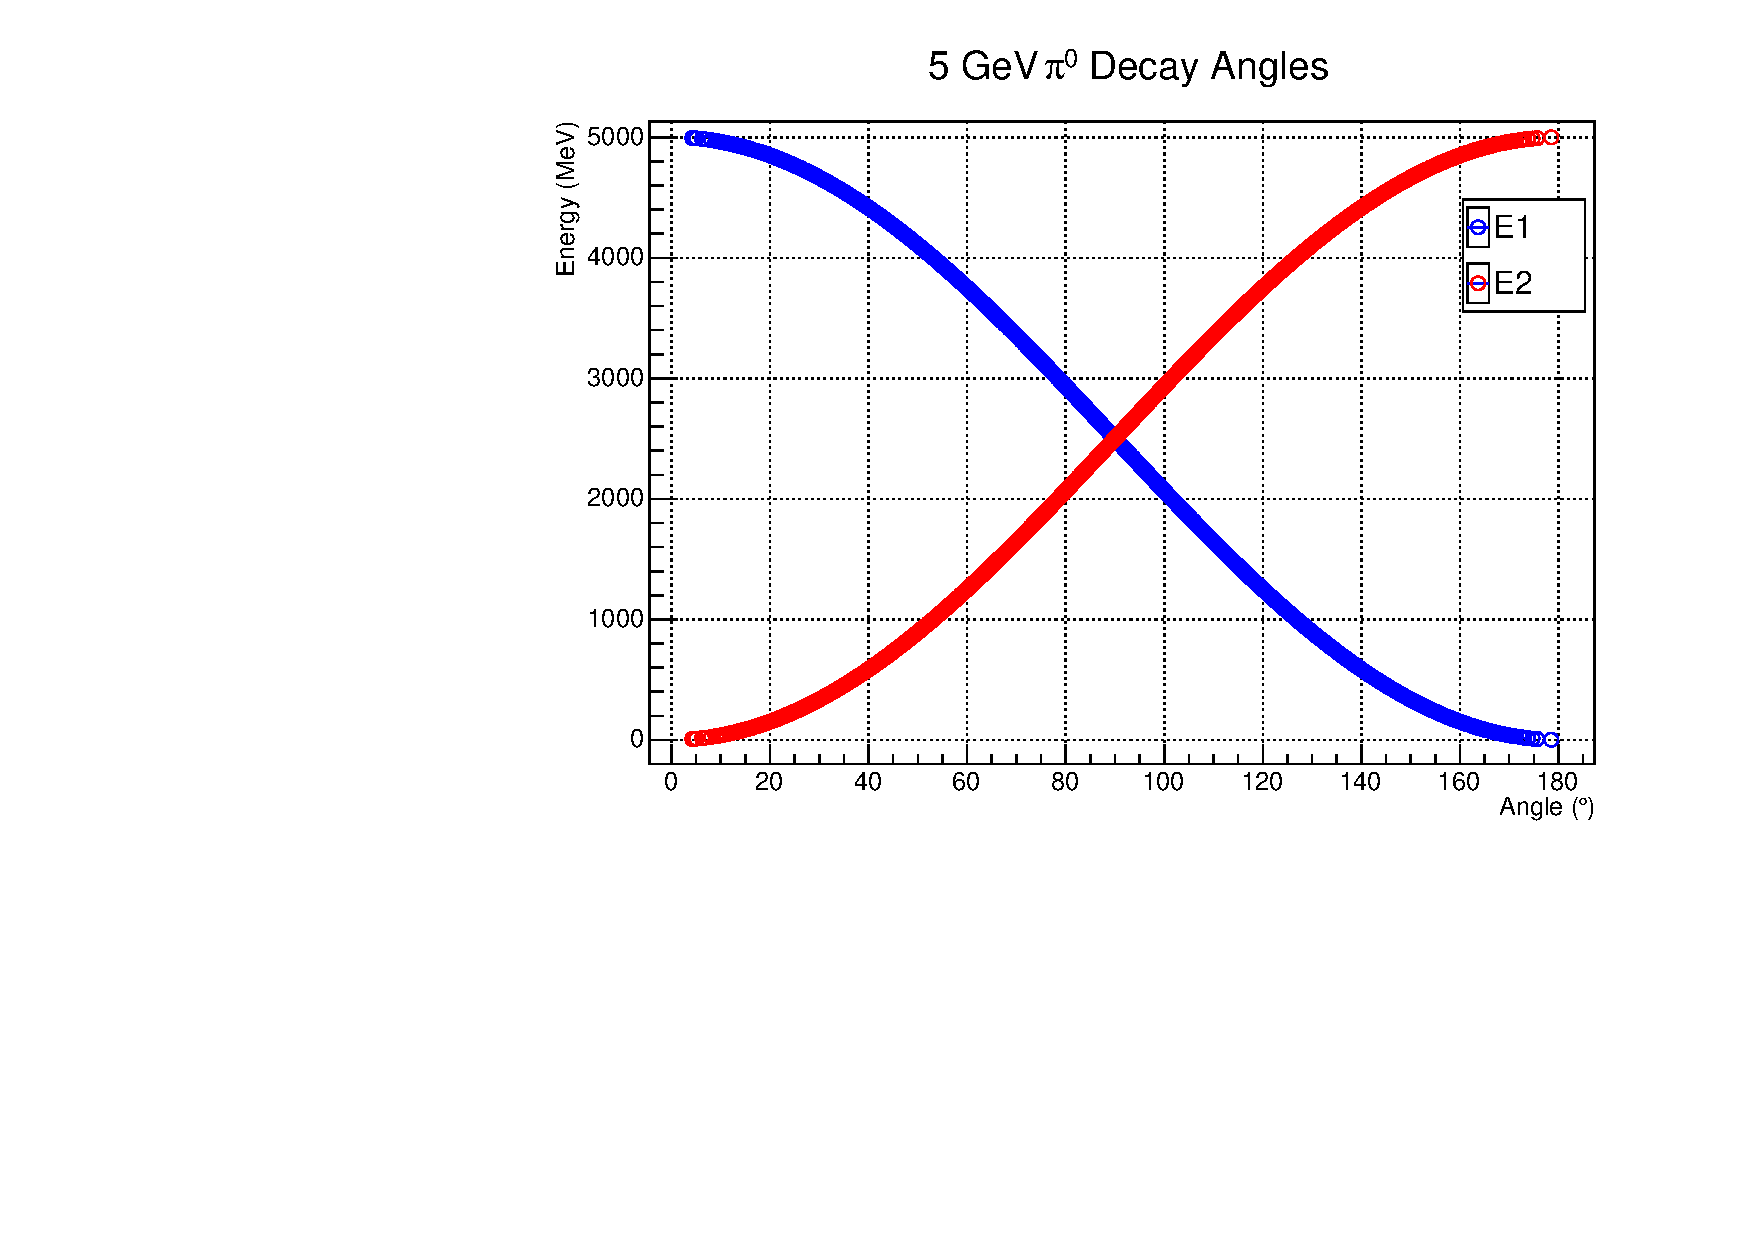
\includegraphics[width=3.in]{decayangles5gev.pdf}}
\caption{ \small{Decay angles of $\pi^0$ for 5 GeV using 1000 iterations. E1 and E2 represent gamma ray 1 and gamma ray 2, respectively. \label{relkinmodel}}}
\end{center}
\end{figure}

The data generated for the decaying $\pi^0$ of momentum 5\,GeV were plotted on figure\,\ref{relkinmodel}. The decay was collected for 1000 iterations, yielding the gamma ray opening angle and the characteristic shape of the data.

\begin{equation}
M=2\sqrt{E_1E_2}\sin\frac{\theta}{2}
\label{mpi}
\end{equation}
Equation\,\ref{mpi} was used to find the $\pi^0$ mass for each of the 1000 iterations at 5\,GeV. The $\pi^0$ mass taken with the average value for 1000 iterations was \boxed{3.327\,\textnormal{GeV}}.


\indent Purely with only the energies and angles, the decay point is not obtainable. Extra parameters to more accurately determine the decay point of $\pi^0$ include, detector distance, coordinate system, additional lengths, and time intervals.



\clearpage





%===========================================CHAPTER 4===============================




\section{Chapter 4}

\begin{table}[h!] 
\caption{Sample table of particle parameters measured by DETSIM. This sample includes an energy resolution of 10\% and 0\,cm spatial resolution.}
    %table caption at the top is standard
\label{t1}   % labels are used to refer to this in the text
 \begin{center}   % center the table on the page
    \begin{tabular}{|c|c|c|c|c|c|} \hline   % tabular environment 
    $\gamma 1$& $\gamma 1$ & $\gamma 1$ & $\gamma 2$& $\gamma 2$ & $\gamma 2$   \\
x$_1$& y$_1$ & E$_1$ & x$_2$& y$_2$ & E$_2$   \\
&    & (MeV) & &    & (MeV)    \\ \hline \hline \hline


60.61   &-7.92  &2618.12    &-73.88 &9.66   &2222.89\\ \hline
-19.23  &-21.18 &4261.38    &0              &0        &0\\ \hline
46.22   &3.44   &3412.53    &-98.01 &-7.29  &1653.78\\ \hline
     \end{tabular}
  \end{center}
\end{table}


\subsection{Question 4.8}
Three trials were conducted at 20\,m to measure the accuracy of the detector, with 10 iterations each\,([6/10],[4/10],[6/10]). The decay point should be located at approximately \boxed{20\,m} for a $\approx$53.3 percent accuracy in detecting decay photons from 5\,GeV/c $\pi^0$ mesons.
\\
\indent To determine the mass of the $\pi^0$ another trial was conducted, but this time with 100 iterations. The accuracy was 52\%\,[52/100]. Using equation\,\ref{mpi}, the mass determined from the angle and energy outputs was \boxed{0.135\,GeV}. The angles were derived using the x and y points and arctan trigonometry with the 20\,m distance.
\\
\indent This detector will be able to reconstruct the mass of the decaying $\pi^0$ with a 0.047\% efficiency.

\subsection{Question 4.9}
The momentum magnitude of the $\pi^0$ is \boxed{4998.18\,\textnormal{MeV}} with a direction in the z-direction with a z-offset of \boxed{3.31\degree}.
\\
\indent The decay point can be deduced by knowing the known mass of the $\pi^0$, but not through deduction with the prior given parameters. The DETSIM program provides the x and y coordinates for the detector ``hit" locations as well as the z-directional offsets, so the directionality can be determined. With the directionality and the magnitude in the detector, trigonometry can be used to traceback the particle to the point of decay.

\subsection{Question 4.11}

The nomenclature for this section will be defined as (energy\,(\%)/spatial\,(cm)) resolution for more intuitive analysis. The following runs were run with 50 iterations each. 

\begin{table}[h!] 
\caption{Accuracies and masses of the DETSIM detector.}
    %table caption at the top is standard
\label{t1}   % labels are used to refer to this in the text
 \begin{center}   % center the table on the page
    \begin{tabular}{|c|c|c|c|} \hline   % tabular environment 
    Resolution& Accuracy& Decaying Particle & Deviation    \\
Parameters& (\%) & Mass   & from (0/0)   \\
(GeV/cm)& &(GeV)        & (\%)    \\ \hline \hline \hline

(0/0)& 52  & 0.1350$\pm$0.3674  & 0.00   \\ \hline
(10/0)& 42 &0.1349$\pm$0.3673 & 0.04   \\ \hline
(20/0) & 60 &0.1337$\pm$0.3656   & 0.97   \\ \hline
(0/1)  & 46 &0.1349$\pm$0.3673   &0.06   \\ \hline
(10/1) & 58  &0.1352$\pm$0.3677   &0.14   \\ \hline
(20/1) & 56  &0.1373$\pm$0.3706   &1.73   \\ \hline
(10/2) & 60  &0.1353$\pm$0.3678   &0.22   \\ \hline
(20/2) & 68 &0.1351$\pm$0.3675   &0.06  \\ \hline
     \end{tabular}
  \end{center}
\end{table}


\indent For a 5 percent determination of the mass of a decaying particle, the data determined a high energy resolution of \boxed{20\,\%} and a spatial resolution of \boxed{2\,cm} are both needed. The accuracy and the relatively low particle deviation from (0/0) shows that in table\,\ref{t1}.



\section{Acknowledgments}
We would like to thank Group\,1 for providing data for question 4.9.

% the following \setlength is to force the bibliography to have no
% paragraph indentations.Can use vairous units--cm are used here.
\setlength{\parindent}{0cm}

\begin{thebibliography}{99}  % the trailing 99 controls some obscure format--just use

\bibitem{1} \url{http://www.phys.hawaii.edu/~shige/phys481L/Particle.txt}    % {\em } for emphasis, \textbf{ } for boldface

\bibitem{2} \url{http://www.phys.hawaii.edu/~shige/phys481L/relkin.pdf}

\bibitem{3} \url{http://www.phys.hawaii.edu/~shige/phys481L/detsim.pdf}
%\bibitem{3} \url{http://pdg.lbl.gov/2012/tables/rpp2012-sum-leptons.pdf}




\end{thebibliography}





\end{document}

